% ----------------------------------------------------------------------------
% Copyright (c) 2016 by Burkhardt Renz. All rights reserved.
% Die Vorlage für eine Abschlussarbeit in der Informatik am Fachbereich
% MNI der THM ist lizenziert unter einer Creative Commons
% Namensnennung-Nicht kommerziell 4.0 International Lizenz.
%
% Id:$
% ----------------------------------------------------------------------------
\chapter{Implementierung}
\label{chapter:Implementierung}

In diesem Kapitel werden Implementierungen von Prototypen gezeigt, die im Kapitel \cref{chapter:Design} besprochen sind. In \cref{section:Instrumentalisierungsbibliothek: Traktor} werden die implementierungsdetails der Instrumentalisierungsbilbiothek \textbf{Traktor} vorgestellt. In \cref{section:Traktor Agent} und in \cref{section:Traktor Registry} die werden die Traktor Services beschrieben. Anschließend werden zwei Anwendungsfälle gezeigt. Der Anwendungsfall des rendering System in \cref{section:Unity Rendering System} und der Anwendungsfall einer verteilten Webanwendung in \cref{section:Webserver Entwicklungsumgebung}

\section{Instrumentalisierungsbibliothek: Traktor}
\label{section:Instrumentalisierungsbibliothek: Traktor}
In diesem Kapitel wird die Implementierung der Instrumentalisierungsbibliothek Traktor vorgestellt. Es wird das Datenmodell umgesetzt, welches in \cref{section:Datenmodell} konzipiert ist und gezeigt inwiefern Traktor die Anforderungen erfüllt.

Traktor ist eine Instrumentalisierungsbibliothek, die sich die OpenTracing API als Vorbild nimmt. Die OpenTracing API ist eine herstellerneutrale instrumentalisierungs API, die unter der Schirmherschafft der \gls{cncfLabel} steht, welches Teil der gemeinnützig agierenden \gls{lfLabel} ist.

Die Traktor Instrumentalisierungsbibliothek beinhaltet zwei wichtie Einheiten. Das ist zum einen der \textbf{Tracer} und zum anderen \textbf{Spans}. 

\textbf{Tracer}\space\space\space Der Tracer ist die zentrale Verwaltungseinheit der Instrumentalisierung. Dieser verwaltet die Verbindung der Anwendungsinstrumentalisierung zu dem Agenten und der Registry. Der Tracer kümmert sich um das Generieren von Spans und die Herstellung von kausalzusammenhängenen zwischen den Spans. Ausserdem stellt der Tracer die Funktionalitäten zur Kontextpropagierung über die Registry bereit. Die Spans sind Darstellungen von ausgeführter Arbeit in einer instrumentalisierten Anwendung. 

\textbf{Span}\space\space\space Die Spans tragen die Daten, die für eine Ordnungsbildung notwendig sind. Das sind zum einen die Zeitstempel der Startzeit und der Endzeit der ausgeführten arbeit, sowie Identifikationsnummer zur identifizierung der Spans. Die Identifizierung muss durch zwei Daten gegeben sein. Die TraceID stellt die zugehörigekeit eines Spans zu einem Trace dar. Die SpanID ist die Nummer, die ein Span innerhalb eines Traces von anderen Spans unterscheidbar macht. Ein Spankontext wird im Span gespeichert. Dieser stellt gegebenenfalls die nötige Relation zu einem Elternspan her. Durch die Verfolgung der Kontextinhalte, lassen sich die Traces rekonstruieren und eine anschließene Analyse beziehungsweise eine Visualisierung durchführen.


\newpage
\begin{landscape}
	\begin{figure}
		\centering
		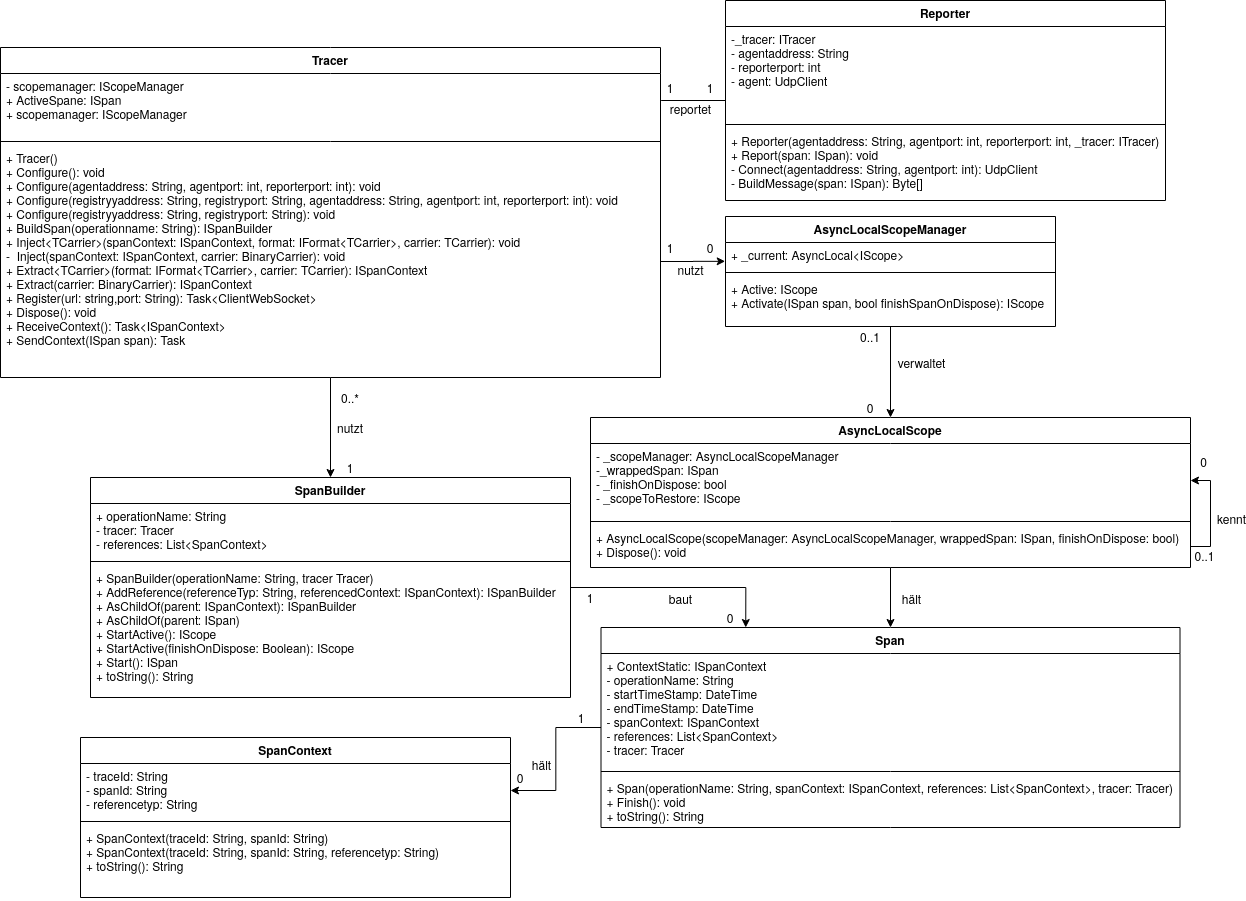
\includegraphics[scale=0.4]{img/Implementierung/TraktorKlassendiagramm.png}
		\caption[Klassendiagramm der Traktor Instrumentalisierungsbibliothek]{Klassendiagramm der Traktor Instrumentalisierungsbibliothek}
		\label{fig:TraktorKlassendiagramm}
	\end{figure}
\end{landscape}

\section{Traktor Agent}
\label{section:Traktor Agent}
\section{Traktor Registry}
\label{section:Traktor Registry}
\section{Unity Rendering System}
\label{section:Unity Rendering System}
\section{ Webserver Entwicklungsumgebung }
\label{section:Webserver Entwicklungsumgebung}
% ----------------------------------------------------------------------------
